%! TEX root = ../main.tex
% ============================================================
% IMMUTABLE — generated automatically, do not edit this block
%   script          : plotter.py::plot_damping_ka
%   plot_type       : damping_ka
%   chapter         : 05
%   panel           : full
%   wind            : allwind
%   amplitude       : 0.1, 0.2, 0.3
%   frequency       : (1.3, 1.6)
%   probes          : None
%   draft           : True
%   n_runs          : 78
%   in_probes_used  : 9373/170+9373/340
%   out_probes_used : 12400/250
%   probe_configs   : march2026_better_rearranging
%
% DATASETS:
%   PROCESSED-20260326-ProbePos4_31_FPV_2-tett6roof-under9Mooring-height100-lowrange
%   PROCESSED-20260327-ProbePos4_31_FPV_2-tett6roof-under9Mooring30-height100-lowrange
%
% SUBFIGURES AVAILABLE:
%   FIGURES/ch05_damping_ka_by_amp_full_10V.pdf
%   FIGURES/ch05_damping_ka_by_amp_full_20V.pdf
%   FIGURES/ch05_damping_ka_by_amp_full_30V.pdf
% ============================================================
\begin{figure}[htbp]
  \centering
  \begin{subfigure}[b]{0.48\linewidth}
    \centering
    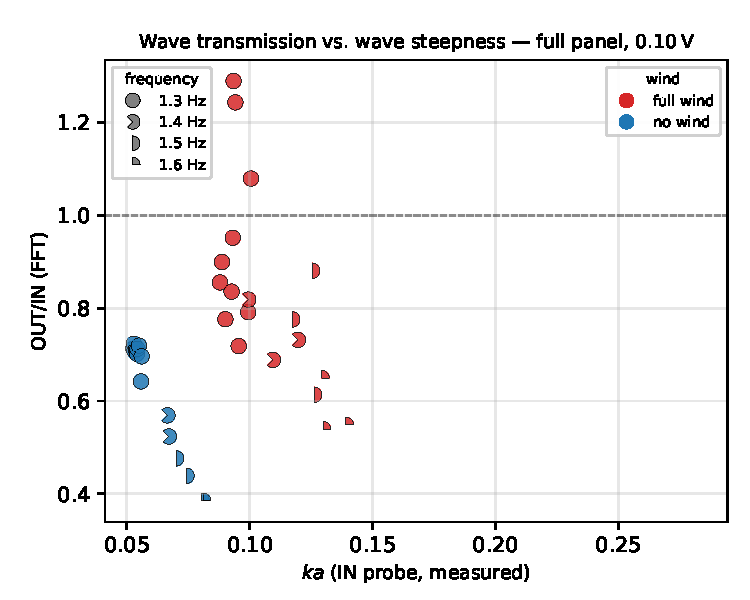
\includegraphics[width=\linewidth]{FIGURES/ch05_damping_ka_by_amp_full_10V.pdf}
    \caption{Full panel, $0.10$\,V}
    \label{fig:TODO_1}
  \end{subfigure}
  \hfill
  \begin{subfigure}[b]{0.48\linewidth}
    \centering
    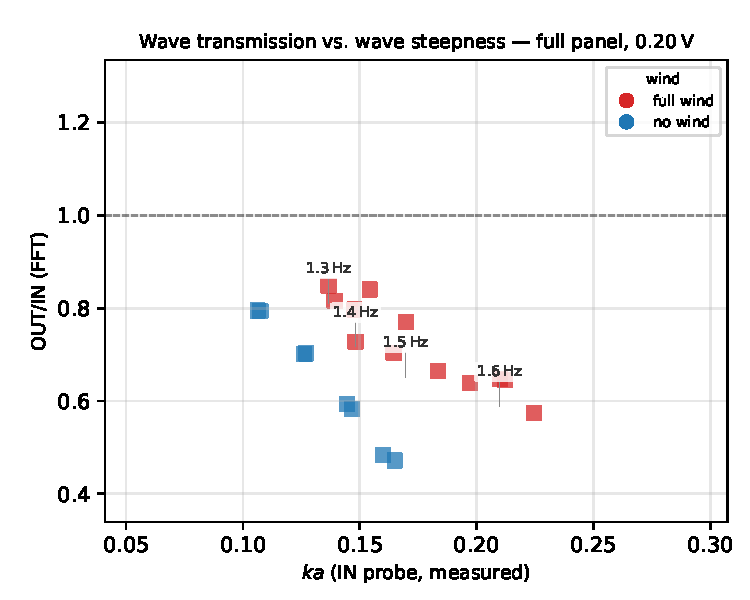
\includegraphics[width=\linewidth]{FIGURES/ch05_damping_ka_by_amp_full_20V.pdf}
    \caption{Full panel, $0.20$\,V}
    \label{fig:TODO_2}
  \end{subfigure}
  \hfill
  \begin{subfigure}[b]{0.48\linewidth}
    \centering
    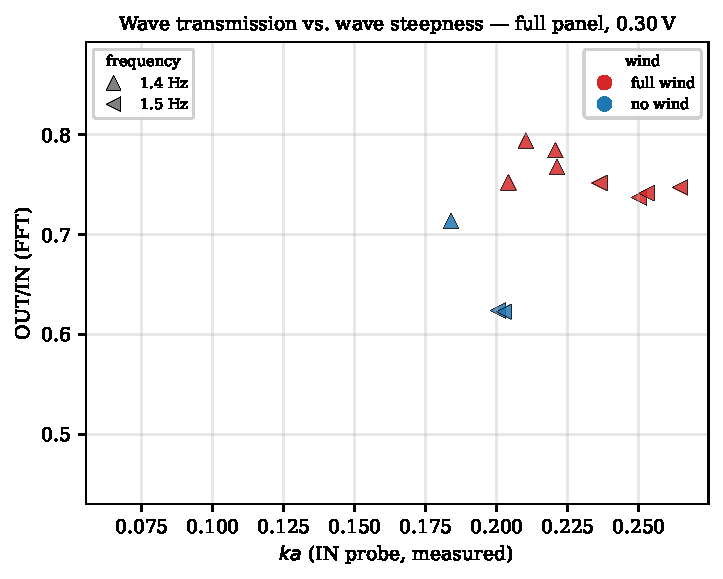
\includegraphics[width=\linewidth]{FIGURES/ch05_damping_ka_by_amp_full_30V.pdf}
    \caption{Full panel, $0.30$\,V}
    \label{fig:TODO_3}
  \end{subfigure}
  \caption[OUT/IN (FFT) vs wave steepness $ka$ using the canonical (per-era mean) IN reference]{
    OUT/IN (FFT) vs wave steepness $ka$ using the canonical (per-era mean) IN reference. Colour: wind. Marker: amplitude. Dashed line: ratio = 1.
  }
  \label{fig:ch05_damping_ka_by_amp}
\end{figure}
